% !TEX TS-program = pdflatex
% !TEX encoding = UTF-8 Unicode

% This is a simple template for a LaTeX document using the "article" class.
% See "book", "report", "letter" for other types of document.

\documentclass[11pt]{article} % use larger type; default would be 10pt

\usepackage[utf8]{inputenc} % set input encoding (not needed with XeLaTeX)

%%% Examples of Article customizations
% These packages are optional, depending whether you want the features they provide.
% See the LaTeX Companion or other references for full information.

%%% PAGE DIMENSIONS
\usepackage{geometry} % to change the page dimensions
\geometry{a4paper} % or letterpaper (US) or a5paper or....
%\geometry{margin=2in} % for example, change the margins to 2 inches all round
%\geometry{left=2.75cm, right=2.75cm, top=3.5cm, bottom=4.5cm}
\geometry{left=3.0cm, right=3.0cm, top=3.5cm, bottom=4.0cm}
% \geometry{landscape} % set up the page for landscape
%   read geometry.pdf for detailed page layout information

\usepackage{graphicx} % support the \includegraphics command and options

% \usepackage[parfill]{parskip} % Activate to begin paragraphs with an empty line rather than an indent

%%% PACKAGES
\usepackage{booktabs} % for much better looking tables
\usepackage{array} % for better arrays (eg matrices) in maths
\usepackage{paralist} % very flexible & customisable lists (eg. enumerate/itemize, etc.)
\usepackage{verbatim} % adds environment for commenting out blocks of text & for better verbatim
\usepackage{subfig} % make it possible to include more than one captioned figure/table in a single float
% These packages are all incorporated in the memoir class to one degree or another...

%%% HEADERS & FOOTERS
\usepackage{fancyhdr} % This should be set AFTER setting up the page geometry
\pagestyle{fancy} % options: empty , plain , fancy
\renewcommand{\headrulewidth}{0pt} % customise the layout...
\lhead{}\chead{}\rhead{}
\lfoot{}\cfoot{\thepage}\rfoot{}

%%% SECTION TITLE APPEARANCE
\usepackage{sectsty}
\allsectionsfont{\sffamily\mdseries\upshape} % (See the fntguide.pdf for font help)
% (This matches ConTeXt defaults)

%%% ToC (table of contents) APPEARANCE
\usepackage[nottoc,notlof,notlot]{tocbibind} % Put the bibliography in the ToC
\usepackage[titles,subfigure]{tocloft} % Alter the style of the Table of Contents
\renewcommand{\cftsecfont}{\rmfamily\mdseries\upshape}
\renewcommand{\cftsecpagefont}{\rmfamily\mdseries\upshape} % No bold!

%%% BibTex packages (url for website references)
\usepackage[english]{babel}
\usepackage[numbers]{natbib}
% \usepackage{url}
% \usepackage{Biblatex}

%For inclusion of hyperlinks
\usepackage{hyperref}
\hypersetup{
    colorlinks=true,
    linkcolor=blue,
    filecolor=magenta,      
    urlcolor=cyan,
}

%BibTex stuff and referencing sections by name 
\urlstyle{same}
\usepackage{nameref} 

%%% END Article customizations

%%% Change distance between bullet points
\usepackage{enumitem}
%\setlist{noitemsep}
\setlist{itemsep=0.2pt, topsep=6pt, partopsep=0pt}
%\setlist{nosep} % or \setlist{noitemsep} to leave space around whole list

%%% For aside comments
\usepackage[framemethod=TikZ]{mdframed}
\usepackage{caption}

%%% AMS math
\usepackage{amsmath}

%%% For differential notation
\usepackage{physics}

%%% For SI unit notation
% Dependencies for siunitx
\usepackage{cancel}
\usepackage{caption}
\usepackage{cleveref}
\usepackage{colortbl}
\usepackage{csquotes}
\usepackage{helvet}
\usepackage{mathpazo}
\usepackage{multirow}
\usepackage{listings}
\usepackage{pgfplots}
\usepackage{xcolor}
\usepackage{siunitx}

%%% User commands
% theorem box
\newcounter{aside}[section]\setcounter{aside}{0}
\renewcommand{\theaside}{\arabic{section}.\arabic{aside}}
\newenvironment{aside}[1][]{%
\refstepcounter{aside}%
\mdfsetup{%
frametitle={%
\tikz[baseline=(current bounding box.east),outer sep=0pt]
\node[anchor=east,rectangle,fill=blue!20]
{\strut Aside~\theaside};}}
\mdfsetup{innertopmargin=10pt,linecolor=blue!20,%
linewidth=2pt,topline=true,%
frametitleaboveskip=\dimexpr-\ht\strutbox\relax
}
\begin{mdframed}[]\relax%
\label{#1}}{\end{mdframed}}

% For titification of tables
\newcommand{\ra}[1]{\renewcommand{\arraystretch}{#1}}

\usepackage{ctable} % for footnoting tables

% Aside environment for personal comments / ideas
%\newcounter{asidectr}

%\newenvironment{aside} 
%  {\begin{mdframed}[style=0,%
%      leftline=false,rightline=false,leftmargin=2em,rightmargin=2em,%
%          innerleftmargin=0pt,innerrightmargin=0pt,linewidth=0.75pt,%
%      skipabove=7pt,skipbelow=7pt]
%  \refstepcounter{asidectr}% increment the environment's counter
%  \small 
%  \textit{Aside \theasidectr:}
%  \newline
%  \relax}
%  {\end{mdframed}
%}
%\numberwithin{asidectr}{section}

% Keywords command
\providecommand{\keywords}[1]
{
  \small	
  \textbf{\textit{Keywords---}} #1
}

% command for oversetting distributed sign with text
\makeatletter % changes the catcode of @ to 11 (i.e. letter)

\newcommand{\distas}[1]{\mathbin{\overset{#1}{\kern\z@\sim}}}%
\newsavebox{\mybox}\newsavebox{\mysim}

\newcommand{\distras}[1]{%
  \savebox{\mybox}{\hbox{\kern3pt$\scriptstyle#1$\kern3pt}}%
  \savebox{\mysim}{\hbox{$\sim$}}%
  \mathbin{\overset{#1}{\kern\z@\resizebox{\wd\mybox}{\ht\mysim}{$\sim$}}}%
}
\makeatother % changes the catcode of @ to 12 (i.e. back to default, other)

% Command for named label for referencing
%\def\namedlabel#1#2{\begingroup
%    #2%
%    \def\@currentlabel{#2}%
%    \phantomsection\label{#1}\endgroup
%}

%%% The "real" document content comes below...

%\title{Modelling photosynthetic parameters via mixed effects models and the Farquhar-van Cammerer-Berry model}
\author{Stephen D. Coleman}
%\date{} % Activate to display a given date or no date (if empty),
         % otherwise the current date is printed 

\begin{document} \pgfplotsset{compat=1.15}
%\maketitle

\begin{titlepage}
\begin{center}
\vspace*{1cm}

\par{\LARGE \textbf{Modelling photosynthetic parameters via mixed effects models and the Farquhar-van Cammerer-Berry model}}

\vspace{0.5cm}
MAT80436

\vspace{1.5cm}

\textbf{Stephen D. Coleman \\ 940309160050}

\vspace{2.8cm}

supervised by \\
\textbf{Gerrit Gort} \\
Biometris, Wageningen University, \\
\textbf{Elias Kaiser} \\
Max Planck Institute of Molecular Plant Physiology, \\
\textbf{Rachel Schipper} \\
Horticulture and Product Physiology, Wageningen University, \\
and \\
\textbf{Anne Elings} \\
Wageningen Plant Research.

%\vspace{1.0cm}


\vfill

A thesis presented for the degree of \\
Master's in Bioinformatics

\vspace{0.8cm}

%		\includegraphics[width=0.4\textwidth]{university}

%			Genetics \\
Wageningen University

\end{center}
\end{titlepage}

\begin{abstract}
The study of the photosynthetic process frequently involves analysis of net assimilation - intercellular CO$_2$ concentration (ACI) curves. These are used in the estimation of key parameters associated with the Farquhar-van Caemmerer-Berry (FvCB) \cite{Farquharbiochemicalmodelphotosynthetic1980} model:
\begin{itemize}
 \item $V_{c_{max}}$: the rate of maximum Rubisco carboxylation;
 \item $J$: electron transport rate;
 \item $R_d$: daytime respiration; and
 \item $g_m$: mesophyll conductance.
\end{itemize}
Accurate, unbiased estimation of these parameters is a non-trivial exercise with the optimal method still a matter of debate within the field \cite{Moualeu-Nganguenewmethodestimate2017}\cite{YinTheoreticalreconsiderationswhen2009}\cite{QianEstimationphotosynthesisparameters2012}. The problem of selecting suitable starting values for a non-linear model is thus complicated by the lack of unanimity on what is a ``good'' estimate of these. The core model we are using to estimate the parameters is based on \citet{YinUsingcombinedmeasurements2009}. This method offers several steps to estimate various parameters rather than attempting estimation in a single step. % and Laisk (NEED REFERENCE - think 1977 paper).

The data collected for the purpose of modelling steady-state photosynthesis is inevitably repeated measurements on individual plants. This leads to correlation between measurements, a fact that violates the assumptions in the fixed effects models used in estimating the parameters of interest \cite{DuursmaPlantecophysPackageAnalysing2015}\cite{BellasioExceltoolderiving2016}. We introduce the use of non-linear mixed effects models in keeping with \citet{QianEstimationphotosynthesisparameters2012} to overcome this issue, and extend on their work by considering more modern versions of the FvCB model.
\end{abstract}
\keywords{ACI curves, parameter estimation, FvCB model, non-linear mixed effects models}

\newpage

\section*{Acknowledgements}
Thanks are due to my supervisors, Gerrit, Elias, Rachel and Anne without whom this project would not have been possible. Gerrit's patience with dealing with me as the primary supervisor was exemplary. He had to explain a few basic parts of the non-linear mixed effect model on more than one occasion. He ensured that the project kept focused and had some conclusion - difficult things to guarantee. Elias provided much needed clarity in the murky world of plant physiology. Rachel arrived at the 11th hour and provided the data we used - a relevant modern dataset. She also provided much cheer and her best efforts in understanding the models we used. Jeremy Harbinson also offered guidance and advice which were appreciated - he pointed us towards the paper by \citet{YinUsingcombinedmeasurements2009} originally. Maikel Verouden was of help, kindly solving several network issues I had within Biometris.

\newpage

%\begin{abstract}
%The study of the photosynthetic process frequently involves analysis of net assimilation - intercellular CO$_2$ concentration (ACI) curves. These are used in the estimation of key parameters associated with the Farquhar-van Caemmerer-Berry (FvCB) \cite{Farquharbiochemicalmodelphotosynthetic1980} model:
%\begin{itemize}
% \item $V_{c_{max}}$: the rate of maximum Rubisco carboxylation;
% \item $J$: electron transport rate;
% \item $R_d$: daytime respiration; and
% \item $g_m$: mesophyll conductance.
%\end{itemize}
%Accurate, unbiased estimation of these parameters is a non-trivial exercise with the optimal method still a matter of debate within the field \cite{Moualeu-Nganguenewmethodestimate2017}\cite{YinTheoreticalreconsiderationswhen2009}\cite{QianEstimationphotosynthesisparameters2012}. The problem of selecting suitable starting values for a non-linear model is thus complicated by the lack of unanimity on what is a ``good'' estimate of these. The core model we are using to estimate the parameters is based on \citet{YinUsingcombinedmeasurements2009}. This method offers several steps to estimate various parameters rather than attempting estimation in a single step. % and Laisk (NEED REFERENCE - think 1977 paper).
%
%The data collected for the purpose of modelling steady-state photosynthesis is inevitably repeated measurements on individual plants. This leads to correlation between measurements, a fact that violates the assumptions in the fixed effects models used in estimating the parameters of interest \cite{DuursmaPlantecophysPackageAnalysing2015}\cite{BellasioExceltoolderiving2016}. We introduce the use of non-linear mixed effects models in keeping with \citet{QianEstimationphotosynthesisparameters2012} to overcome this issue, and extend on their work by considering more modern versions of the FvCB model.
%\end{abstract}
%\keywords{ACI curves, parameter estimation, FvCB model, non-linear mixed effects models}

\section{Theory}
\subsection{FvCB model}
The brilliant realisation of \citet{Farquharbiochemicalmodelphotosynthetic1980} was that the net photosynthesis rate, $A$, of C$_3$ plants could be accurately modeled at the leaf level as being in one of two steady-state systems. In \emph{Rubisco activity limited net photosynthesis rate} ($A_c$), the net rate of photosynthesis is limited by the properties of the enzyme ribulose 1.5 biphosphate carboxylase/oxygenase (Rubisco) (we assume saturating levels of the substrate, RuBP). In the second we assume that it is the substrate that determines the rate of assimilation; specifically its regeneration rate. Hence the second state is referred to as RuBP-regeneration limited or \emph{electron transport limited net photosynthesis rate} ($A_j$)\cite{YinUsingcombinedmeasurements2009}. We prefer the latter name for being a more clear difference for readers unfamiliar with the biochemical constituents of the photosynthesis cycle.

\begin{figure}[h]
\centering
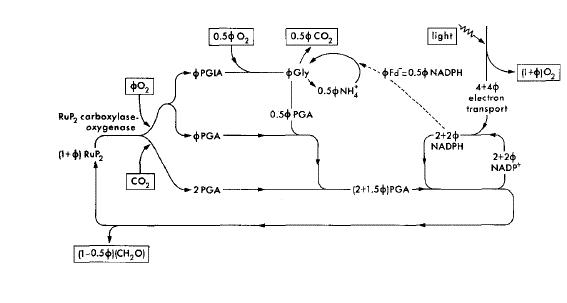
\includegraphics[scale=0.75]{Images/fvcb_model}
\caption{Diagram of metabolic pathways described in the FvCB model.}
\label{fig:fvcb}
\end{figure}

\subsubsection{Some assumptions} \label{Assumptions}
For parsimony's sake, we make several simplifying assumptions regarding the homogeneity of conditions within the leaf. We disregard any gradient of temperature ($T$) or O$_2$ within the leaf. According to \citet{CaemmererBiochemicalmodelsleaf2000}, these, specifically within C$_3$ species, are unlikely to be important. Due to the thinness of leaves we also assume an equal distribution of light to all chloroplasts within the leaf; however, it has been shown that under certain conditions these assumptions and their corollary, that photosynthesis itself is homogeneous across the leaf, do not hold. Non-uniform photosynthesis can occur and this will affect the gas-exchange measurements and their interpretation \cite{TerashimaAnatomynonuniformleaf1992}.

We account for the \emph{Kok effect} in our modelling. This is a physiological effect where in low light (typically $0-20\SI{}{\micro \mol \per \m \squared \per \s}$ \cite{TcherkezTrackingoriginsKok2017}) conditions the quantum yield of net photosynthesis is higher than at higher levels of incident light. Thus, the net assimilation recorded tends to escape description by our model. This is a well documented effect \cite{TcherkezTrackingoriginsKok2017}\cite{SharpKokEffectQuantum1984}\cite{HeskelBringingKokeffect2013} and hence in some the low light data the first point (we will often consider increasing intercellular carbon dioxide ($C_i$) or light intensity ($I$) as pseudo-time in our descriptions) will be ignored in our models.

Several parameters require estimation, and some measurements are not feasible for the majority of experiments. For these we need either a starting value that is our initial best guess (feasible in C$_3$ species, less so in C$_4$) or a correction to some related measurement. We will  show the reasoning behind our choices below.

\subsubsection{Rubisco activity limited net photosynthesis rate}
The photosynthetic carbon reduction (PCR) and photorespiratory carbon oxidation (PCO) cycles are linked by an enzyme common to both, RuBP \cite{Farquharbiochemicalmodelphotosynthetic1980}. In the PCO cycle, $0.5$ mol of CO$_2$ is released, thus:
\begin{equation} \label{net_assimilation_raw}
A = V_c - 0.5 V_o - R_d
\end{equation}
Where:
\begin{itemize}
 \item $V_c$ is the rate of carboxylation; and
 \item $V_o$ is the rate of oxygenation.
\end{itemize}
We have from \citet{FarquharModelsdescribingkinetics1979} (assuming RuBP binding first in the reaction):
\begin{align} \label{V_c}
V_c &= V_{c_{max}}\frac{C_c}{C_c+K_c\left(1 + O/K_o\right)}\cdot\frac{R}{R + K^\prime_r} \\
V_o &= V_{o_{max}}\frac{O}{O+K_o\left(1 + C_c/K_c\right)}\cdot\frac{R}{R + K^\prime_r}
\end{align}
Where:
\begin{itemize}
 \item $V_{c_{max}}$ is the maximum velocity of the carboxylase;
 \item $V_{o_{max}}$ is the maximum velocity of the oxygenase;
 \item $O$ is the partial pressure of oxygen in the chloroplast;
 \item $K_c$ is the Michaelis-Menten constant for CO$_2$;
 \item $K_o$ is the Michaelis-Menten constant for O;
 \item $R$ is the concentration of free RuBP; and
 \item $K^\prime_r$ is the effective Michaelis-Menten constant for RuBP.
\end{itemize}
This leads to the ratio of oxygenation to carboxylation:
\begin{equation} \label{ratio_oxygenation_carboxylation}
\phi = \frac{V_o}{V_c} = \frac{V_{o_{max}}}{V_{c_{max}}}\cdot\frac{O/K_o}{C_c/K_c}
\end{equation}
We also have that the velocity of carboxylation, at saturating levels of RuBP, ($W_c$) is given by \cite{GrantTestsimplebiochemical1989}:
\begin{equation} \label{RuBP_satuarted_carboxylation_rate}
W_c = V_{c_{max}} \frac{C_c}{C_c + K_c (1 + O / K_o)}
\end{equation}
Note that this arises from setting the RuBP component of \eqref{V_c} to 1.
The compensation point for $C_c$ at which there is no net assimilation, $\Gamma_*$, is given by \cite{Farquharbiochemicalmodelphotosynthetic1980}:
\begin{equation} \label{gamma_star}
\Gamma_* = \frac{K_c O}{2 K_o}\cdot \frac{V_{o_{max}}}{V_{c_{max}}}
\end{equation}
Relating \eqref{net_assimilation_raw}, \eqref{ratio_oxygenation_carboxylation}, \eqref{RuBP_satuarted_carboxylation_rate} and \eqref{gamma_star} we have:
\begin{equation} \label{rubisco_limited_photosynthesis}
A_c = V_{c_{max}} \frac{C_c - \Gamma_*}{C_c+K_c(1+O/K_o)}-R_d
\end{equation}
This is the Rubisco-limited rate of assimilation, assuming saturation of RuBP.

\subsubsection{Electron transport limited net photosynthesis rate}
The physiology of this model is somewhat more complex, involving analysis of the cycle for the production of NADPH \cite{Farquharbiochemicalmodelphotosynthetic1980}. A thorough understanding of this is beyond the scope of this project, but we recommend the reader to the original paper \cite{Farquharbiochemicalmodelphotosynthetic1980} and \citet{CaemmererBiochemicalmodelsleaf2000}. We are content to state that when $A$ is limited by RuBP regeneration:
\begin{equation} \label{RuBP_photosynthesis}
A_j = J\frac{C_c - \Gamma_*}{4C_c + 8\Gamma^*}-R_d
\end{equation}
Where $J$ is the rate of electron transport (and hence electron transport limited net photosynthesis rate). This equation arises using assumptions that RuBP regeneration is limited because of insufficient NADPH and implicitly assumes $100\%$  linear e$^-$ transport. \citet{SharkeyFittingphotosyntheticcarbon2007} recommend the use of $4$ and $8$ in the denominator based on the number of electrons required for NADP$^+$ reduction; however this is not always the case; values of 4.5 and 10.5 also occur in the literature and less frequently we see 4 and 9.33 (see \cite{SharkeyFittingphotosyntheticcarbon2007}\cite{YinUsingcombinedmeasurements2009}\cite{YinC3C4photosynthesis2009}). These different values arise from different assumptions about the complexity of linear electron (e$^-$) rate. The disagreement over pairs $\{4.5, 10.5\}$ or $\{4, 9.33\}$ arise due to further disagreement about deeper levels of this system that are a source of some discussion in the literature (\cite{CaemmererBiochemicalmodelsleaf2000}\cite{YinUsingcombinedmeasurements2009}) but are less of interest to us. To allow for this disagreement we use default values of 4 and 8 in our R model, but the functions incorporating this aspect of the model allow the user to input their own version of these coefficients.

\subsubsection{TPU limited net photosynthesis rate} \label{TPU_limited_photosynthesis}
Other models extend to different cases (such as C$_4$ species) or to encompass more physiologically limiting factors (such as triose phosphate utilization (\emph{TPU}) in the synthesis of starch and sucrose). TPU is required at one third the rate of CO$_2$ fixation. If this is not acquired, the level of free phosphate declines and the rate of photosynthesis is limited. When this is limit is imposed, it can be seen that photosynthesis becomes independent of the ratio of oxygenation to carboxylation \cite{ThomasD.SharkeyPhotosynthesisIntactLeaves1985}. \citet{SharkeyFittingphotosyntheticcarbon2007} model this \emph{TPU limited net photosynthesis rate} ($A_p$) using the following equation:
\begin{equation} \label{TPU_photosynthesis}
A_p = 3TPU - R_d
\end{equation}
Where $TPU$ is the rate of triose phosphate utilization. This extension is only relevant under high $C_i$ and $I$ environments and is normally modeled as a upper bound on $A$. We do not include this in our model, but recommend extending the model to this scenario in later versions. From \citet{CaemmererBiochemicalmodelsleaf2000} we know that this model is too simple for the reality, please see \citet{HarleyimprovedmodelC31991} an extension. However, this linear assumption is normally considered sufficient as the majority of ACI curves will have only the most extreme measurements affected by this mode. As a result of this (that TPU limited photosynthesis \eqref{TPU_photosynthesis} only emerges in extreme conditions) we ignore it for now but recommend inclusion of this additional case in any extensions to our work.

\subsubsection{FvCB summary}
For the final model, our actual assimilation rate is calculated by combining these individual curves. The curve fitted is:
\begin{equation} \label{FvCB_equation}
A = \min \left \{A_c, A_j\right \}
\end{equation}
Where:
\begin{itemize}
 \item $A_c$ is the Rubisco activity limited net photosynthesis rate calculated from \eqref{rubisco_limited_photosynthesis}; and
 \item $A_j$ is the electron transport limited net photosynthesis rate calculated from \eqref{RuBP_photosynthesis}.
% \item $A_p$ is the TPU limited net photosynthesis rate calculated from \eqref{TPU_photosynthesis}.
\end{itemize}
%\section{FvCB model}
%The ubiquitous model in the field is the FvCB model, a steady-state biochemical description of the net assimilation rate. It is based on the realisation of a number of limiting factors,

\subsubsection{Relating $C_i$ to $C_c$}
One of the driving factors in net assimilation rate ($A$) is the level of CO$_2$ present at the Rubisco site of carboxylation in the chloroplasts ($C_c$) \cite{VonCaemmererSteadystatemodelsphotosynthesis2013}. Estimation of the intercellular CO$_2$ partial pressure ($C_i$) is based on gas exchange measurements and is not a matter of controversy. Less well established is estimation of $C_c$ \cite{YinTheoreticalreconsiderationswhen2009}.  We can relate $C_i$ to $C_c$ using Flick's first law relating the diffusive flux to the concentration  under steady-state assumptions. We have:
\begin{equation} \label{Flicks_law}
J = -D\dv{\phi}{x}
\end{equation}
Where:
\begin{itemize}
 \item $J$ is the diffusion flux;
 \item $D$ is the diffusion coefficient;
 \item $\phi$ is the concentration; and
 \item $x$ is position.
\end{itemize}
Please note that the notation used in \eqref{Flicks_law} is the generic notation used normally in describing Flick's Law and will not be referring to these terms after this subsection. From this we can consider $A$ as our flux, and the difference between $C_c$ and $C_i$ as our gradient in concentration:
\begin{equation} \label{Flicks_law_step_2}
A = -D(C_c - C_i)
\end{equation}
The diffusion conductance between the substomatal cavities and the chloroplasts is $g_m$, the mesophyll conductance \cite{NiinemetsImportancemesophylldiffusion2009}. Hence we can write \eqref{Flicks_law_step_2} as:
\begin{equation} \label{Flicks_law_photosynthesis_form}
A = g_m(C_i - C_c)
\end{equation}
Or equivalently:
\begin{equation} \label{Ci_Cc_relationship}
C_c = C_i - \frac{A}{g_m}
\end{equation}
Thus we can calculate $C_c$, the variable relevant to our models, using $C_i$.

\subsubsection{Mesophyll conductance}
To estimate values of $C_c$ we need to have an estimate of $g_m$. \citet{HarleyTheoreticalConsiderationswhen1992a} propose a model for this:
\begin{equation} \label{eqn_g_m}
g_m = \frac{A}{C_i - \frac{\Gamma_* \left[J + 8 (A + R_d) \right]}{J - 4 (A + R_d)}}
\end{equation}

\subsubsection{Light dependence of electron transport rate}
We can relate $J_{max}$ to the incident irradiance by empirical equation:
\begin{equation} \label{J_J_max_relationship}
 \theta J^2 - J\left (I_2 + J_{max}\right ) + I_2J_{max} = 0
\end{equation}
Where:
\begin{itemize}
 \item $I_2$ is the useful light absorbed by photosystem two (PSII);
 \item $J$ is the electron transport;
 \item $J_{max}$ is the maximum electron transport; and
 \item $\theta$ is an empirical curvature factor (often around 0.7 \cite{EvansPhotosynthesisnitrogenrelationships1989}).
\end{itemize}
$I_2$ is related to total incident irradiance $I$ (sometimes referred to as the Photosynthetically Active Radiation, $PAR$, in the literature) by:
\begin{equation} \label{I_2_def}
I_2 = I \times \textrm{abs}(1-f)/2
\end{equation}
The coefficient of $I$ here is often collapsed into a lump term, $\alpha$ which is estimated. 
Where:
\begin{itemize}
 \item abs is the absorptance of leaves (commonly around 0.85 \cite{CaemmererBiochemicalmodelsleaf2000});
 \item $f$ is the correction for the spectral quality of light (approximately 0.15 \cite{EvansDependenceQuantumYield1987}); and
 \item The 2 in the denominator is due to the split of light between photosystems I and II (PSI and PSII respectively).
\end{itemize}
We can thus solve for $J$ in the usual way \cite{QianEstimationphotosynthesisparameters2012}\cite{YinC3C4photosynthesis2009}:
\begin{equation} \label{nonrectangular_hyperbola}
J = \frac{\alpha \cdot I + J_{max} - \sqrt{\left (\alpha \cdot I + J_{max}\right )^2 - 4 \cdot \alpha \cdot \theta \cdot I \cdot J_{max}}}{2  \cdot\theta}
\end{equation}
Equations of this form are referred to as \emph{non-rectangular hyperbola functions}, a fact which mention due to references to this term in the literature.

\subsubsection{Lump parameter, $s$}
\citet{YinUsingcombinedmeasurements2009} propose use of a lump parameter, $s$, in their photosynthesis model. This parameter is a function of several variables describing the photosystems I and II. Specifically it is:
\begin{equation} \label{lump_parameter_def}
s = \rho_2\beta\left(1 - \frac{f_{pseudo(b)}}{1 - f_{cyc}}\right)
\end{equation}
Where:
\begin{itemize}
 \item $\rho_2$ is the proportion of light absorbed by photosynthetic pigments partitioned to PSII (\citet{YinUsingcombinedmeasurements2009} suggest this is in the range of 0.5 but suggest some caution in using this value. We suspect that the 2 in the denominator of \eqref{I_2_def} corresponds to this coefficient. Again the literature finds a new name and symbol for a pre-existing concept);
 \item $\beta$ is the absorptance by leaf photosynthetic pigments (abs in \eqref{I_2_def});
 \item $f_{pseudo(b)}$ is the fraction of electrons at PSI that follow the basal pseudocyclic e$^-$ flow; and
 \item $f_{cyc}$ is the fraction of electrons at PSI that follow cyclic transport around PSI.
\end{itemize}
Note that $f$ in \eqref{I_2_def} corresponds to $ \frac{f_{pseudo(b)}}{1 - f_{cyc}}$.

This highlights the problem rampant in the photosynthesis modeling literature - this appears to be another way of representing the previously defined lump parameter $\alpha$ with more detail (more aspects of the photosystems are accounted for). However, it is a completely different set of symbols and no acknowledgment of overlap despite $\alpha$ being far more common in preceding papers. Possibly this is not problematic for plant physiologists, but we suspect that this has lead to confusion and could be avoided by either continuity in symbols or else directly acknowledging past preferences in the current form.

\subsubsection{Relative CO$_2$/O$_2$ specificity factor for Rubisco, $S_{c/o}$}
The relative CO$_2$/O$_2$ specificity factor for Rubisco, $S_{c/o}$, is used in calculating both $\Gamma_*$ and $J$ in the linear part of the light response curve \cite{YinUsingcombinedmeasurements2009}. It is estimated using the linear part of the high and low oxygen ACI curves. \citet{YinUsingcombinedmeasurements2009} propose a relationship between the net rate of photosynthesis in the linear part of the high and low oxygen ACI curves defined by:
\begin{align}
A_h = (A_l + R_d) \frac{b_h}{b_l} - \left( \frac{O_h - O_l}{2 S_{c/o}} + C_{i_l} - C_{i_h} \right) b_h - R_d
\end{align}
By solving for $S_{c/o}$ we find:
\begin{equation} \label{Sco_eqn}
S_{c/o} = \frac{(O_h - O_l)}{2 ((A_l + R_d) / b_l - (A_h + R_d) / b_h - (C_{i_l} - C_{i_h}))}
\end{equation}
In these equations the subscripts refer to which dataset the parameter is from, $l$ for the low oxygen dataset and $h$ for the high oxygen set respectively. An explanation of these different datasets is sketched below in section \ref{datasets}. $b_h$ and $b_l$ are the slope of the linear part of the ACI curve under the different oxygen conditions.

\subsubsection{CO$_2$ compensation point in the absence of $R_d$}
The $C_i$-based CO$_2$ compensation point in the absence of $R_d$, $\Gamma_*$, is point at which the plant's production of $CO_2$ has a net value of $0$; i.e. it is consuming as much CO$_2$ in photosynthesis as it produces through photorespiration (as $R_d$, the day respiration, is respiratory CO$_2$ release other than by photorespiration). We let:
\begin{equation} \label{Gstar_eqn}
\Gamma_* = \frac{O}{2S_{c/o}}
\end{equation}

\subsubsection{Temperature dependency}
The dependency of the rate of carboxylation and oxygenation of Rubisco is reflected in the temperature dependency of $A$. As a rate dependent upon temperature, we consider using Arrhenius functions, equations of the form:
\begin{equation} \label{arrhenius_eqn_kelvin}
x(T) = k \cdot \exp \left(-\frac{E_a}{R \cdot T}\right)
\end{equation}
Where:
\begin{itemize}
 \item $x(T)$: the temperature dependent rate we are interested in;
 \item $k$: the rate coefficient;
 \item $E_a$: the activation energy, the kinetic energy of substrate required for the reaction to occur;
 \item $R$: the universal gas constant ($\SI{8.314}{\J \per \K \per \mol}$); and
 \item $T$: temperature (in Kelvin).
\end{itemize}
As most photosynthesis measurement are recorded in $\SI{}{\celsius}$, and specifically use a default value of $\SI{25}{\celsius}$, we transform the equation to this scale. In this case we have:
\begin{equation} \label{arrhenius_eqn}
x(T^\prime) = k' \cdot \exp \left(-\frac{(25 - T')E_a}{298.15 R \cdot (273.15 + T')}\right)
\end{equation}
Where $T'$, $k'$ are the relevant form of $T$, $k$ for a scale centred on $T = \SI{25}{\celsius}$. As we will not be using the Kelvin scale again, we denote $T = T'$, $k = k'$.
Many reactions in photosynthesis are reversible, with differing activation energies depending on the direction of the reaction. Thus the net activation energy may vary depending on the ratio of forward to backward reactions. This means that the Arrhenius function \eqref{arrhenius_eqn} is only semi-empirical, but it does allow easy comparison between studies.

Another frequently used method to describe a dependency on temperature is the \emph{$Q_{10}$ temperature coefficient}. This is a measure of of the rate of  change of a system as a result of raising the temperature by $\SI{10}{\celsius}$. It is calculated:
\begin{equation} \label{Q10_gen}
Q_{10} = \left ( \frac{R(T_2)}{R(T_1)} \right )^{\SI{10}{\celsius}/(T_2 - T_1)}
\end{equation}
Where:
\begin{itemize}
 \item $Q_{10}$ is the factor by which the reaction rate increases when temperature is raised by $\SI{10}{\celsius}$;
 \item $T_i$ is the temperature for the $i^{th}$ measurement; and
 \item $R(T_i)$ is the rate of the reaction at temperature $T_i$.
\end{itemize}
Alternatively we can write this in the form:
\begin{equation}
R(T_2) = R(T_1) Q_{10}^{(T_2 - T_1)/\SI{10}{\celsius}}
\end{equation}
Again, this general form is of less interest as we have a specific, default temperature of $\SI{25}{\celsius}$ for which we are quite well informed. Hence, we use:
\begin{equation} \label{Q10}
R(T) = R(\SI{25}{\celsius})Q_{10}^{(T-25)/10}
\end{equation}
This function allows us to relate values given at the temperature $T = \SI{25}{\celsius}$ to more general temperatures. This was not integrated into the final project here (temperatures where approximately $\SI{25}{\celsius}$), but it is information to be aware of in attempting to generalise some of the models to different conditions. We give the required $Q_{10}$ in table \ref{photosynthesis_params_T25} for several key parameters.

\subsubsection{Model parameters}
Many parameters can be assigned \emph{a priori}, leaving only the estimation of a small number of key variables. The kinetic constants of rubisco vary very little among C$_3$ species such that one can use the same $K_c$, $K_o$ and $\Gamma_*$ across all members of this category \cite{CaemmererBiochemicalmodelsleaf2000}. This means that the only parameter requiring estimation for Rubisco is the maximal Rubisco activity, $V_{c_{max}}$. 
%For this parameter:
%\begin{displayquote}
%``Rubisco has a molecular weight of $\SI{550}{\kilo \dalton}$ and eight catalytic sites per molecule.  Thus, with a catalytic turnover rate of $\SI{3.5}{\per \second}$ per site, $\SI{1}{\gram \per \metre \squared}$ of Rubisco has a $V_{c_{max}}$ of $\SI{51}{\micro \mol \per \metre \squared \per \second}$ when Rubisco sites are fully carbamylated.'' \cite{CaemmererBiochemicalmodelsleaf2000}
%\end{displayquote}

For RuBP-limited photosynthesis, we need to solve for $J_{max}$ as we can relate this to $J$ by equation \eqref{nonrectangular_hyperbola}. According to \citet{Walcroftresponsephotosyntheticmodel1997}, the ratio $J_{max} : V_{c_{max}}$ is expected to vary from $2$ to $1.4$ across the range $[\SI{8}{\celsius}, \SI{30}{\celsius}]$.

\citet{EvansCarbonDioxideDiffusion1996} recommend setting $g_m =  0.0045V_{c_{max}}$. Other values can be seen, with an assumption of $g_m = \infty$ used frequently, but this is controversial and can lead to biased estimates of $V_{c_{max}}$ and $J_{max}$ \cite{YinTheoreticalreconsiderationswhen2009}. Specific plants in specific conditions can see diverging values, but we feel this is a sufficient initial value.

This means that if we have an empirically driven initial value for $V_{c_{max}}$ we can initialise all our parameters to some default temperature, however these relationships vary with temperature, the relationship of which we state below.

We use table \ref{photosynthesis_params_T25} for our initial values of photosynthetic parameters in our model. We can combine these with \eqref{Q10} to calculate initial values for our model across a range of temperatures. Many of the values in table \ref{photosynthesis_params_T25} can be found in \citet{CaemmererBiochemicalmodelsleaf2000}.

\ctable[
cap = Parameters, botcap,
caption = {Photosynthetic parameters and their activation energy for $T=\SI{25}{\celsius}$},% \cite{CaemmererBiochemicalmodelsleaf2000}},
label = nowidth,
pos = !htb,
label = photosynthesis_params_T25
] {lcccc} {
\tnote[a]{The first value is appropriate when an internal diffusion conductance is included; the second value should be used if the internal conductance is not included (i.e. $g_m = \infty$) and $C_c$ is assumed to equal $C_i$.}
\tnote[b]{From \citet{Farquharbiochemicalmodelphotosynthetic1980}}
\tnote[c]{From \citet{EvansCarbonDioxideDiffusion1996}}
}{ \FL
Parameter & \emph{unit} & Value & E $(\SI{}{\kilo \J \per \mol})$ & $Q_{10} (T = \SI{25}{\celsius})$ \ML
$K_c$ & $\SI{}{\micro \bar}$ & $260$ or $404$\tmark[a] & $59.36$\tmark[b] & $2.24$ \NN
$K_o$ & $\SI{}{\milli \bar}$ & 179 or $248$\tmark[a] & 35.94 & 1.63 \NN
$\Gamma_*$ & $\SI{}{\micro \bar}$ & 38.6 or 37\tmark[a] & 23.4 & 1.37 \NN
$V_{c_{max}}$ & $\SI{}{\micro \mol \per \m \squared \per \s}$ & 80 & 58.52 & 2.21 \NN
$V_{o_{max}}$ & $\SI{}{\micro \mol \per \m \squared \per \s}$ & 20  & 58.52 & 2.21 \NN
$R_d$ & $\SI{}{\micro \mol \per \m \squared \per \s}$ & $0.8 - 1.6$ & 66.4 & 2.46 \NN
$J_{max}$ & $\SI{}{\micro \mol \per \m \squared \per \s}$ & $100 - 160$ & 37 & 1.65 \NN
$g_m$ & $\SI{}{\micro \mol \per \m \squared \per \s}$ & $0.35 $\tmark[c] or $\infty$ & & \NN
%H & $\SI{}{\kilo \J \per \mol}$ &  & 220 & \NN
%S & $\SI{}{\J \per \K \per \mol}$ & & 710 & \NN
$\alpha$ or $s$ & & 1.2 & \NN
$\theta$ & &  0.7 & \LL
}
The assumption that $g_m = \infty$,  equivalent to $C_c = C_i$ is now considered redundant but would severely change these values. We include a sample of this impact to enable comparison with older papers and research.

\subsection{Mixed-effects models}
\subsubsection{Linear mixed-effects models}
Traditional parametric models incorporate only \emph{fixed effects}. That is, they have a set of parameters describing with the entire population. For example, consider a system of $n \in \mathbb{N}$ observations of dependent variable, $Y=(y_1,\ldots,y_n)$, and the $n \times p$ matrix of associated independent variable measurements, $X=\left\{x_{i,j}\right\}$ for $i \in [1,n], j \in [1,p]$ for some $p \in \mathbb{N}$, and a $p$-vector of weights, $\beta$, represented:
\begin{equation} \label{linear_model}
Y = X \beta  + \epsilon
\end{equation}
Here $X$ is assumed to contain a column of $1$'s in the first position (hence the +1 in the description of its dimensionality) and $\epsilon$ is the $n$-vector of associated errors. We assume that $\epsilon_i \distras{iid} \mathcal{N}(0,\sigma^2)$ for $i = (1,\ldots,n)$.  If we consider the intuitive case of \emph{biological} and \emph{technical replicates}, where we have $n$ biological replicates and for the $i^{th}$ sample $m_i$ associated technical replicates. As each of the $m_i$ measurements is on the same sample we expect there to be a non-negligible correlation between the $m_i$ technical replicates for each $i$. The model in \eqref{linear_model} does not allow for the within group effects due to the correlation between technical replicates. Consider the simplest possible model for the fixed effects model including only the intercept:
\begin{equation}
y_{i,j} = \beta + \epsilon_{i,j}, \hspace{4mm} i = 1,\ldots,n, \hspace{4mm} j = 1,\ldots,m_i
\end{equation}
Some of this model's limitations become apparent if one considers the case of unbalanced data. Continuing the previous example of biological and technical replicates, consider the case that $m_i \neq m_j$ for any $i, j \in (1,\ldots,n)$. In this case the model is skewed by the within sample data rather than by the true observations, the biological replicates. A possible solution is the inclusion of a individual intercept for each group of technical replicates, accommodating the within-sample variability, or \emph{random effects}:
\begin{equation}
y_{i,j} = \beta_i + \epsilon_{i,j}, \hspace{4mm} i = 1,\ldots,n, \hspace{4mm} j = 1,\ldots,m_i
\end{equation}
While this better describes the observed data, it has certain inherent flaws; most  notably the number of parameters scales linearly with the number of observations and the model only describes the measurements included in the sample. Consider as a solution a combination of these models, containing both a sample mean, $\beta$, and a random variable for each group representing the deviation from the population mean, $b_i$, i.e. a \emph{mixed effects} model:
\begin{equation} \label{lme_model}
y_{i,j} = \beta + b_i + \epsilon_{i,j}, \hspace{4mm} i = 1,\ldots,n, \hspace{4mm} j = 1,\ldots,m_i
\end{equation}
The linear mixed effects model described in \eqref{lme_model} contains information at both a population level (in the fixed effects) but also at the individual level (in the random effects).

For now we assume $b_i \distras{iid} \mathcal{N}(0,\sigma_b^2) $ for $i = 1,\ldots,n$. This means that the variance of the observations is divided into two parts, $\sigma_b^2$ for the biological variability and $\sigma^2$ for the technical variability:
\begin{equation} \label{hierarchical_model}
b_i \distras{iid} \mathcal{N}(0,\sigma_b^2), \hspace{4mm} \epsilon_{i,j} \distras{iid} \mathcal{N}(0,\sigma^2)
\end{equation}
The assumption of normality can be modified if deemed inappropriate and it is possible to generalise the model to allow for heteroscedasticity.

The $b_i$ are called \emph{random effects} as they are associated with the experimental unit and selected at random from the population of interest (at least in theory, obviously there are limitations on this particularly in the area of medicine) They represent that the effect of choosing the sample $i$ is to shift the mean expression of $Y$ from $\beta$ to $\beta + b_i$ - i.e. they effect a deviation from an overall mean. Technical replicates share the same random effect $b_i$ and are correlated. The covariance between technical replicates on the same experimental unit is $\sigma^2_b$; this corresponds to a correlation of $\frac{\sigma^2_b}{\left(\sigma^2_b + \sigma^2\right)}$.

\subsubsection{Non-linear mixed effects models}
Non-linear mixed effects models, also known as \emph{non-linear hierarchical models}, are an extension to the more traditional linear mixed effects models. They are used in scenarios where all of the following features are present \cite{DavidianNonlinearmodelsrepeated2003a}:
\begin{enumerate}  \label{when_nlme}
 \item Repeated observations of a continuous variable on each of several \emph{experimental units} (in our case these are individuals, thus individual is considered equivalent to empircial unit in the following section) over time or another condition (e.g. measurements at given heights on a tree) (the \emph{condition variable});
 \item We expect the relationship between the response variable and the condition variable to vary across individuals; and
 \item Availability of a scientifically relevant model characterising the behaviour of the individual response in terms of meaningful parameters that vary across individuals and dictate variation in patterns of condition-response (for us this will be the Farquhar-van Cammerer-Berry model).
\end{enumerate}
The final point from the list in \ref{when_nlme} is where the non-linear aspect is introduced. This is often a mechanistic function describing a physical or chemical system (for example in toxicokinetics physiologically-based pharmacokinetics models are used or HIV dynamics in ``precision medicine''); that is the model is described by by meaningful, interpretable parameters rather than being an empirical best fit. It is expected that the mechanistic model will better describe data beyond the range of the measurements used here (whereas an empirical fit might describe the data over the range captured in the measurement data but then misbehave woefully beyond these boundaries).

The analysis tends to have the goal of understanding one or more of the following:
\begin{enumerate}
 \item The ``typical'' behaviour of the phenomena (i.e. mean or median values) represented by the model parameters;
 \item The variation of these parameters, and hence the phenomena, between individuals; and
 \item If some of the variation is inherently associated with individual characteristics.
\end{enumerate}
Individual level prediction can also be of interest (e.g. in medical treatment with highly individual reaction), but is less relevant to this project. From the individual level we are interested in investigating the level of variation between individuals and questioning if this is sufficiently small to allow the ``all-purpose'' models generally used in photosynthesis describing the parameters and systems of interest.

Consider an experiment involving repeated measurements of some response variable, $Y$, across a condition variable $T$ for $n$ individuals. Each individual's characteristics are recorded in $A$ (this is assumed to be time-independent measurements, like an individual's height over the course of a drugs trial) and possible additional initial conditions in $U$ (for example the dose of a drug the individual was receiving at time $t=0$). Let $y_{i,j}$ denote the $j$th measurement of the response under condition $t_{i,j}$, $j = 1,\ldots,n_i$, for individual $i$, $i = 1,\ldots,n$ with additional initial conditions $u_i$. Thus:
\begin{equation}
\begin{array}{ll}
Y &= \left(y_1,\ldots,y_n\right) \\
y_i &= \left(y_{i,1},\ldots,y_{i,n_i}\right) \\
T &= \left(t_1,\ldots,t_n\right) \\
t_i &= \left(t_{i,1},\ldots,t_{i,n_i}\right) \\
A &= \left(a_1,\ldots,a_n\right) \\
U &= \left(u_1,\ldots,u_n\right)
\end{array}
\end{equation}
We denote $x_{i,j} = \left(t_{i,j}, u_i\right)$. Often $T$ is time and $U=\emptyset$, but it might be the case that each $t_{i,j}$ is a $p_1$-vector of measurements and $u_i$ is a $p_2$-vector such that $p_1 + p_2 = p$, returning to the notation of \eqref{lme_model}. The assumption that the triplets $(y_i,u_i,a_i)$ are independent across $i$ is often included to reflect the belief that individuals are unrelated (this will hold for us, but might require more thought in other situations). For some function $f$ regulating the within-individual behaviour defined by a vector of parameters $\beta_i$ unique to individual $i$, we have:
\begin{equation} \label{stage1_individual_model}
y_{i,j} = f\left(x_{i,j}, \beta_i\right) + \epsilon_{i,j}, \hspace{4mm} j = 1,\ldots,n_i
\end{equation}
For us this will be the Farquhar-van Cammerer-Berry model of steady-state photosynthesis. We assume that $\mathbb{E}\left(\epsilon_{i,j}|u_i,\beta_i\right)=0$ and $\epsilon_{i,j} \distras{iid} \mathcal{N}(0,\sigma^2)$ for all $i, j$ (the assumption of normality can be relaxed, but this extension exceeds the reach of this project). This model in \eqref{stage1_individual_model} is called the \emph{individual level model}. To model the population parameters we consider $d$, a $p$-dimensional function depending on an $r$-vector of fixed parameters, or \emph{fixed effects}, $\beta$, and a $k$-vector of \emph{random effects}, $b_i$, associated with individual $i$:
\begin{equation} \label{stage1_population_model}
\beta_i = d\left(a_i,\beta,b_i\right), \hspace{4mm} i = 1,\ldots,n
\end{equation}
Here, the \emph{population model} in \eqref{stage1_population_model} describes how $\beta_i$ varies among individuals due to both individual attributes $a_i$ and biological variation in $b_i$. We assume that the $b_i$ are independent of the $a_i$, i.e.:
\begin{equation}
\begin{array}{l}
\mathbb{E}(b_i|a_i) = \mathbb{E}(b_i) = 0 \\
\mathbb{V}ar(b_i|a_i) = \mathbb{V}ar(b_i) = D
\end{array}
\end{equation}
Here, $D$ is an unstructured covariance matrix and is common to all $i$. It characterises the degree of unexplained variation in the elements of $\beta_i$ and associations among them; the ubiquitous assumption is $b_i \sim \mathcal{N}(0,D)$.

% However, if this set of assumptions regarding the conditional distribution of $b_i$ on $a_i$ is found to be insufficient, then $b_i \sim \mathcal{N}\left(0,D(a_i)\right)$ is frequently used.

In \eqref{stage1_population_model}, $\beta_i$ is considered to have an associated random effect, reflecting the belief that each component varies non-negligibly in the population even after systematic relationships with subject characteristics are accounted for. It may happen that ``unexplained'' variance in a component of $\beta_i$ may be very small in magnitude relative to that in the remaining elements. In this situation it is common to drop the negligible quantity entirely. This lacks biological sense as each parameter is part of the ``scientifically relevant model'' and thus is unlikely to have no associated unexplained variation. Hence, one must recognise that this omission of an element of $\beta_i$ is adopted to achieve numerical stability in fitting rather than to reflect belief in perfect biological consistency across individuals and analyses in the literature to determine whether elements of $\beta_i$ are fixed or random effects should be interpreted so.

\subsection{Our model} \label{subsect_model}
Much of the preceding concepts and theory make for very pleasant reading, but we consider it useful to explicitly state our mixed-effects model and it's assumptions in one place.

First, recall the FvCB model \eqref{FvCB_equation}:
\begin{align}
A &= \min \left \{A_c, A_j\right \} \\
 &= FvCB(C_c, \Gamma_*, I, K_c, K_o, O, J_{max}, V_{c_{max}}, \alpha, \theta, R_{d_i})
\end{align}
Where $A_c$ and $A_j$ are two curves describing separate biochemical limits on the rate of photosynthesis, from \eqref{rubisco_limited_photosynthesis} and \eqref{RuBP_photosynthesis} respectively:
\begin{align}
A_c &= V_{c_{max}} \frac{C_c - \Gamma_*}{C_c+K_c(1+O/K_o)}-R_d \\
A_j &= J\frac{C_c - \Gamma_*}{4C_c + 8\Gamma_*}-R_d
\end{align}
Furthermore, from \eqref{nonrectangular_hyperbola}:
\begin{equation}
J = \frac{\alpha \cdot I + J_{max} - \sqrt{\left (\alpha \cdot I + J_{max}\right )^2 - 4 \cdot \alpha \cdot \theta \cdot I \cdot J_{max}}}{2  \cdot\theta}
\end{equation}
We plug this into \eqref{stage1_individual_model} for each of our experimental effects (in Rachel Schipper's data, SIDE and TREATMENT) in line with \citet{BatesComputationalMethodsMultilevel}. Thus, we have:
\begin{itemize}
 \item Our response variable, $Y$, is net photosynthesis rate, $A$; 
 \item Our individual level function, $f(\cdot)$, is $FvCB(\cdot)$;
 \item Our measured condition variables, $X$, are $C_c, \Gamma_*, I, K_c, K_o$, and $O$; and
 \item Our fixed effects, $\beta$, are $J_{max}, V_{c_{max}}, \alpha, \theta$ and $R_d$.
\end{itemize}
Notice that $U=\emptyset$. Therefore our individual-level model is:
\begin{equation} \label{nlme_fvcb_model}
\begin{array}{ll}
&A_{i,j} = FvCB(C_{c_{i,j}}, \Gamma_{*_{i,j}}, I_{i,j}, K_c, K_o, O_{i,j}, J_{max_i}, V_{c_{max_i}}, \alpha_i, \theta_i, R_{d_i}) + \epsilon_{i,j} \\
&\epsilon_{i,j} \distras{iid} \mathcal{N}(0,\sigma^2) \\
&\mathbb{E}\left(\epsilon_{i,j}|  J_{max_i}, V_{c_{max_i}}, \alpha_i, \theta_i, R_{d_i}\right) = 0
\end{array}
\end{equation}
For our specific version of \eqref{stage1_population_model}, we cannot know in advance what kind of model we will use. This will be based on the ability of different models to converge. We expect, given the paucity of data that we will have a diagonal covariance structure with 0's in the non-diagonal entries imposed on our mixed effects model (as we expect that there is not enough data for more flexible formats to converge). This corresponds to a statement of independence between random effects which may not be the ideal assumption, and with this in mind we will attempt other formats. However we do know that our photosynthetic parameters of interest ($J_{max}, V_{c_{max}}, \alpha, \theta$ and $R_d$) will all be represented in this aspect of the model to consider each individual plant with unique photosynthetic parameters.

\section{Methods}
The methods entailed hereafter are based upon those described by \citet{YinUsingcombinedmeasurements2009} except for the inclusion of mixed-effects models which is, insofar as the author is aware, only previously used in \cite{QianEstimationphotosynthesisparameters2012}. The method described in \cite{YinUsingcombinedmeasurements2009} uses several different datasets to estimate the parameters of interest over several steps. We acknowledge the flaw of this disjoint model which does not accumulate error but instead uses the point estimates in each succeeding step with no error accumulation. If this work is extended upon this is probably the area which most requires improvement, i.e. conversion to a full joint model. We suspect that this should also enable ease of convergence as the point estimates used in any given step might be wrong and restrict the current estimate from moving to the correct subspace of the possible solution space.

The data has been produced by Rachel Schipper as part of her PhD. It is a two-sided photosynthesis experiment; plants (with individual tags) are grown under two treatments (denoted A1 and A2). Measurements are taken from each side of the plants (adaxial or AD and abaxial or AB). The treatment effect is long term - the plants acclimatise to this; the side effect is instantaneoue - a measurement is taken from a side of the leaf.

We have five datasets available for this method. For each dataset we have the same 12 individual plants present.
\begin{enumerate} \label{datasets}
 \item \emph{LRC1}: Repeated measurements for plants acclimatised to increasing values of light intensity ($I$) at constant intercellular CO$_2$ ($C_i$) and atmospheric (i.e. $\SI{210}{\micro \mol}$) O$_2$;
 \item \emph{LRC2}: Repeated measurements for plants acclimatised to increasing values of $I$ at constant CO$_2$ and low (i.e. $\SI{20}{\micro \mol}$) O$_2$;
 \item \emph{LRC2-F}: as LRC2 with the addition of measurements taken using fluorescence;
 \item \emph{ACI1}: Repeated measurements for plants acclimatised to increasing values of $C_i$ at constant $I$ and atmospheric O$_2$; and
 \item \emph{ACI2}: Repeated measurements for plants acclimatised to increasing values of $C_i$ at constant $I$ and low O$_2$.
\end{enumerate}
The method is to calculate or estimate various parameters in individual steps.
\begin{enumerate}
 \item Calculate lump parameter $S$ and $R_d$ using the datasets LRC2 and LRC2-F;
 \item Using the results of the previous step and LRC2-F, estimate J for the low light data;
 \item Calculate the relative CO$_2$/O$_2$ specificity factor for Rubisco, $S_{c/o}$, using the ACI1 and ACI2 datasets by \eqref{Sco_eqn};
 \item Using the value of $S_{c/o}$ from the previous step, calculate $\Gamma_*$ by \eqref{Gstar_eqn};
 \item Calculate $g_m$ using \eqref{eqn_g_m};
 \item Calculate $C_c$ values for each observation via \eqref{Ci_Cc_relationship}; and
 \item Using all of the values previously estimated, estimate $V_{c_{max}}$ and $J_{max}$ using the ACI1 and LRC1 datasets and the model described in \ref{subsect_model}.
\end{enumerate}

\subsection{Estimating $R_d$ and $s$}
We use the relationship proposed by \citet{YinUsingcombinedmeasurements2009} allowing for individual values for each plant. This regresses $A$ on $\frac{1}{4}\phi I$ using a linear mixed effect (LME) model. This combines information from LRC2 and LRC2F (the $\phi$ parameter is measured used flourescence, hence the need for LRC2F). The intercept of the model is $R_d$ and the slope is $s$. It is assumed that $R_d$ and $s$ are constant for each plant regardless of conditions and can thus be used in all datasets for each plant.

\subsection{Estimating $J$ in low-light conditions}
$J$ can be estimated in low light conditions for the linear part of the LCR curve. The calculation is:
\begin{equation}
J = sI \phi_{PSII}
\end{equation}

\section{Results}
\subsection{$R_d$ and $s$}
The estimates of $R_d$ and $s$ are shown in figures \ref{fig:lme_rd} and \ref{fig:lme_s} respectively. We notice that the values estimated are generally positive, which is required for these parameters. However, the standard error (s.e.) on the estimate of $R_d$ does include negative values. We notice that the estimate of $R_d$ is not precise in comparison to $s$ (the point estimates are on the same order of magnitude, but the associated errors are not).

\ctable[
cap = lme_parameters, botcap,
caption = {Estimate of parameters, $R_d$ and $s$},% \cite{CaemmererBiochemicalmodelsleaf2000}},
label = nowidth,
pos = !htb,
label = params_est
] {cccccc} {} { \FL
Side & Treatment & $R_d$ & $R_d$ s.e & $s$ & $s$ s.e \ML
AB & A1 & 0.09 & 0.20 & 0.36 & 0.02 \NN
AD & A1 & 0.10 & 0.26 & 0.46 & 0.03 \NN
AB & A2 & 0.30 & 0.40 & 0.38 & 0.04 \NN
AD & A2 & 0.38 & 0.20 & 0.40 & 0.04 \ML
}

Only consider the linear part of LRC2 and LRC2F we were obliged to include only points for $I \in [30, 100]$ (see Appendix \ref{appendix:lcr_linear}). This reduced the dataset for each individual to three points as shown in figures \ref{fig:lme_fit_ab} and \ref{fig:lme_fit_ad}.

\begin{figure}[h]
\centering
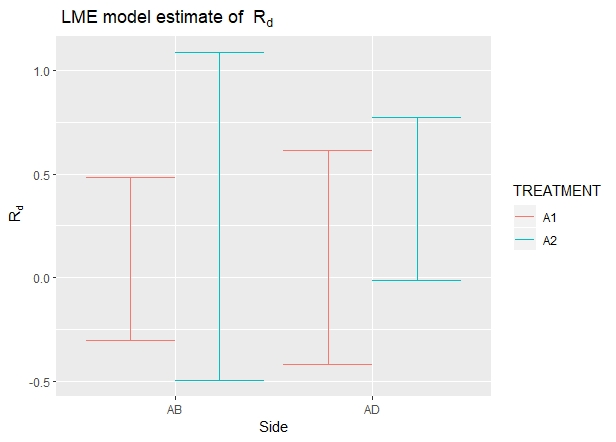
\includegraphics[scale=0.80]{Images/lme_estimate_rd}
\caption{LME model estimates of $R_d$ for treatment and side effects.}
\label{fig:lme_rd}
\end{figure}

\begin{figure}[h]
\centering
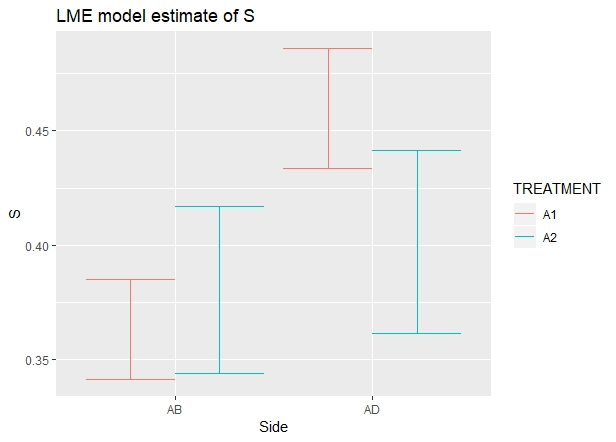
\includegraphics[scale=0.80]{Images/lme_estimate_s}
\caption{LME model estimates of $s$ for treatment and side effects.}
\label{fig:lme_s}
\end{figure}

\begin{figure}[h]
\centering
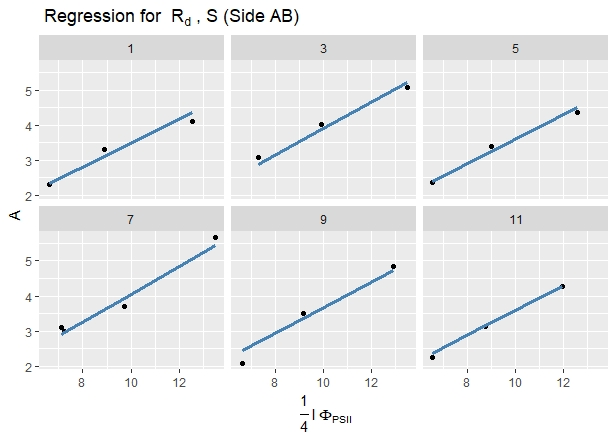
\includegraphics[scale=0.75]{Images/rd_s_ab}
\caption{Model fit for LME model regressing $A$ on $\frac{1}{4} I \phi_{PSII}$ for side AB and treatment A1 faceted by individual plant ID.}
\label{fig:lme_fit_ab}
\end{figure}

\begin{figure}[h]
\centering
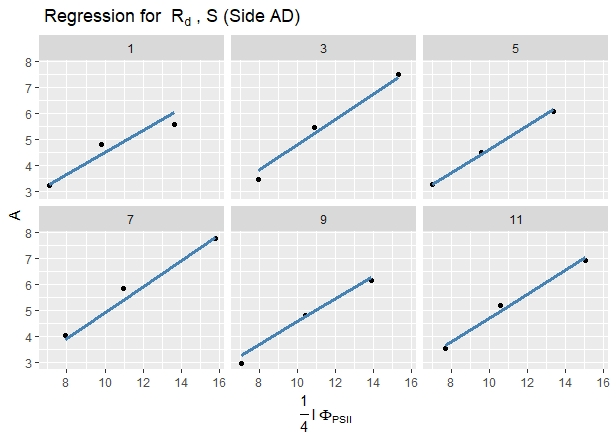
\includegraphics[scale=0.75]{Images/rd_s_ad}
\caption{Model fit for LME model regressing $A$ on $\frac{1}{4} I \phi_{PSII}$ for side AD and treatment A1 faceted by individual plant ID.}
\label{fig:lme_fit_ad}
\end{figure}

\subsection{$S_{c/o}$}
We include boxplots showing the range of values calculated for $S_{c/o}$ across different side and treatment effects for each individual in figures \ref{fig:sco_ab} and \ref{fig:sco_ad}. The median values are given in table \ref{sco_median}.

\ctable[
cap = sco_medians, botcap,
caption = {Median estimated values of $S_{c/o}$ for each side / treatment combination},% \cite{CaemmererBiochemicalmodelsleaf2000}},
label = nowidth,
pos = !htb,
label = sco_median
] {ccc} {} { \FL
Side & Treatment & $S_{c/o}$ \ML
AB & A1 & 1.46  \NN
AD & A1 & 1.71  \NN
AB & A2 & 1.45  \NN
AD & A2 & 1.60 \ML
}

\begin{figure}[h]
\centering
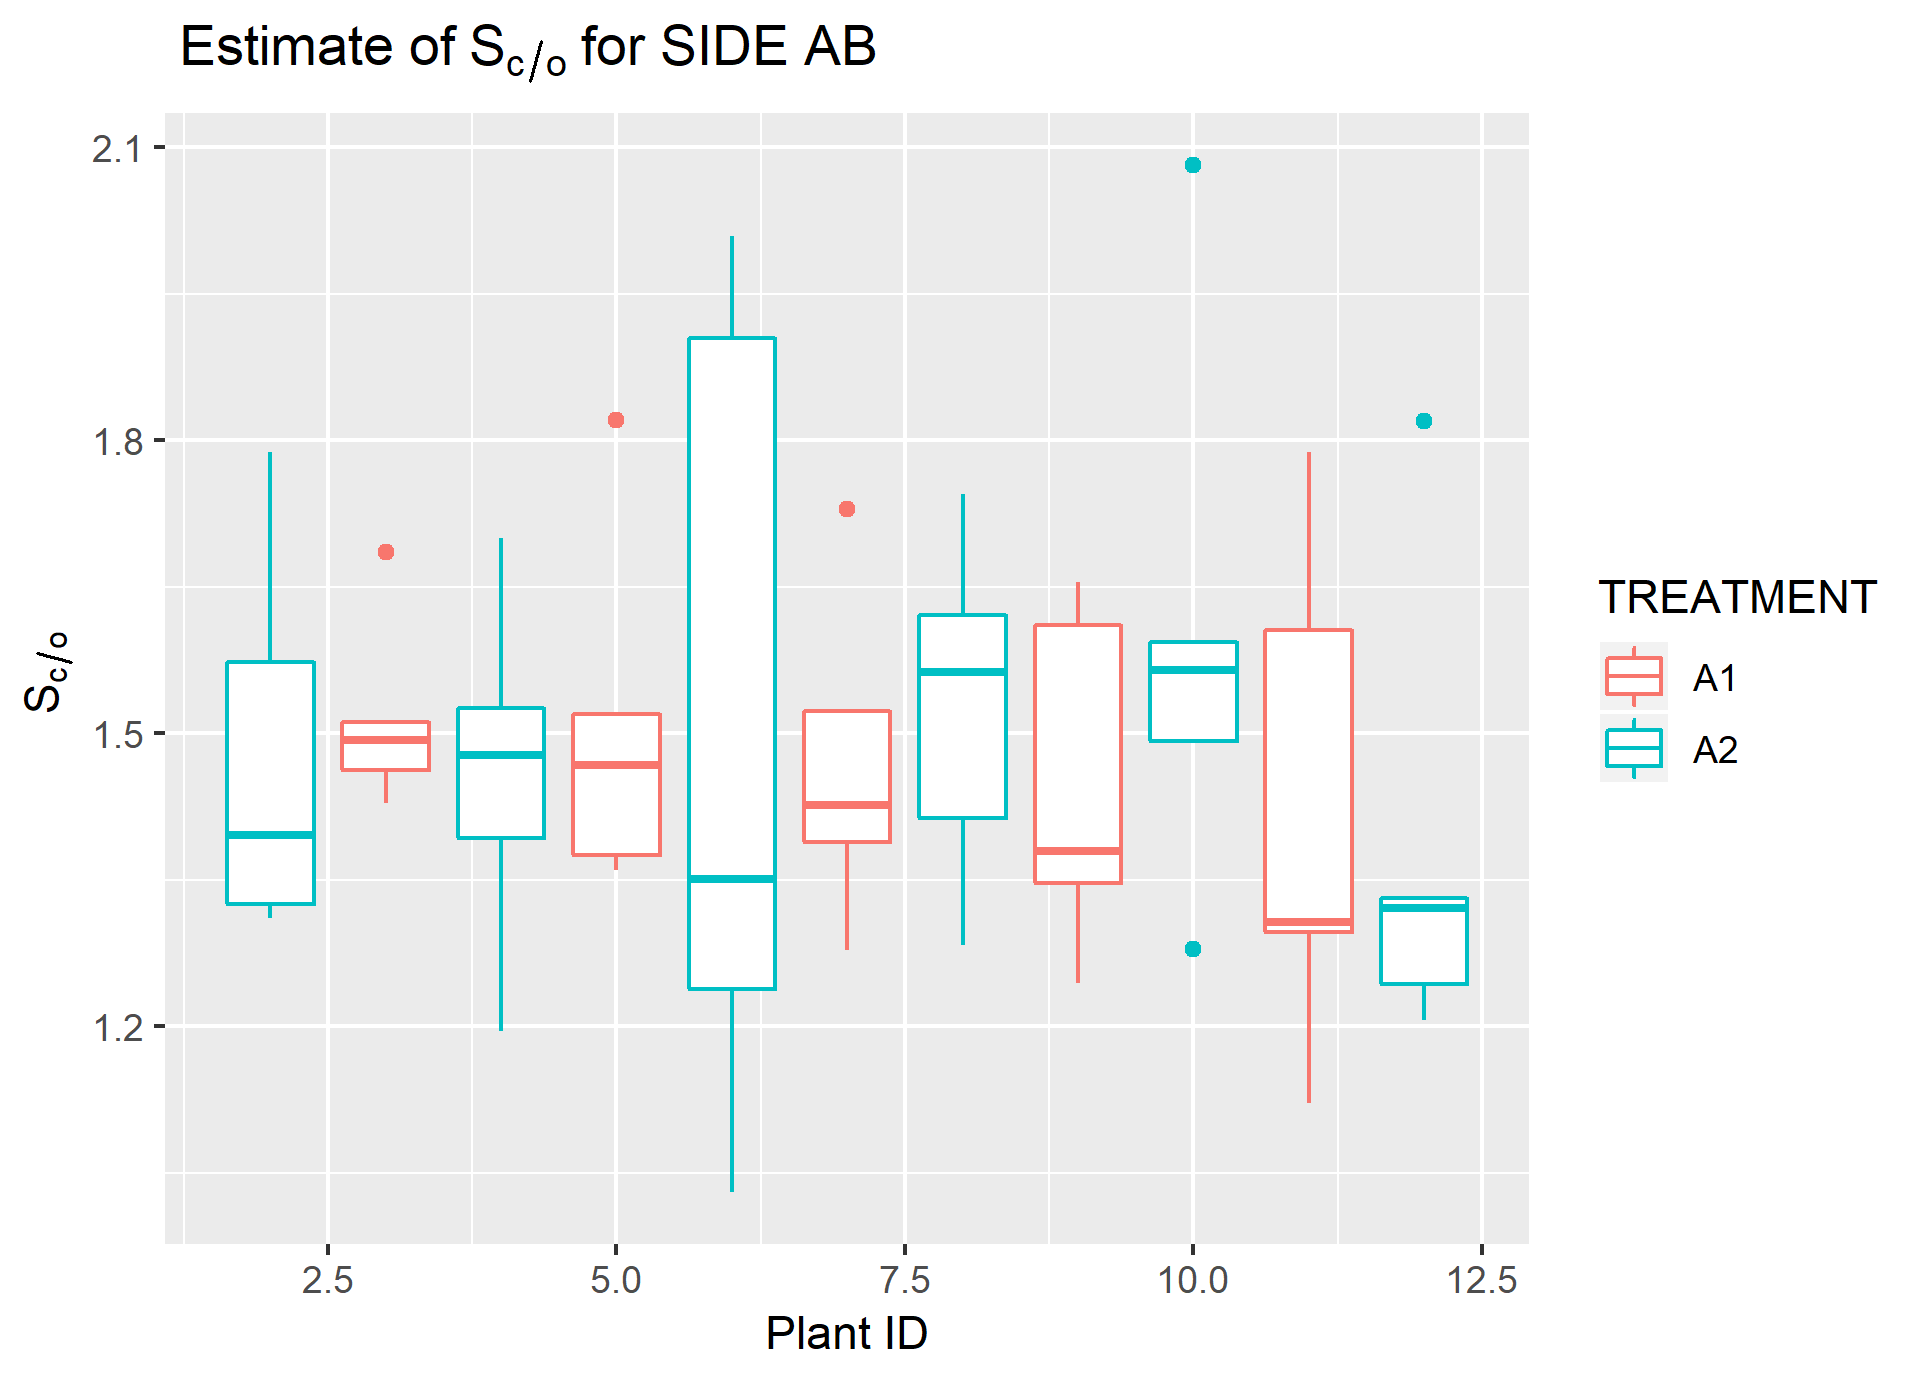
\includegraphics[scale=0.75]{Images/sco_boxplot_ab}
\caption{Range of values for $S_{c/o}$ for side measurement of AB.}
\label{fig:sco_ab}
\end{figure}

\begin{figure}[h]
\centering
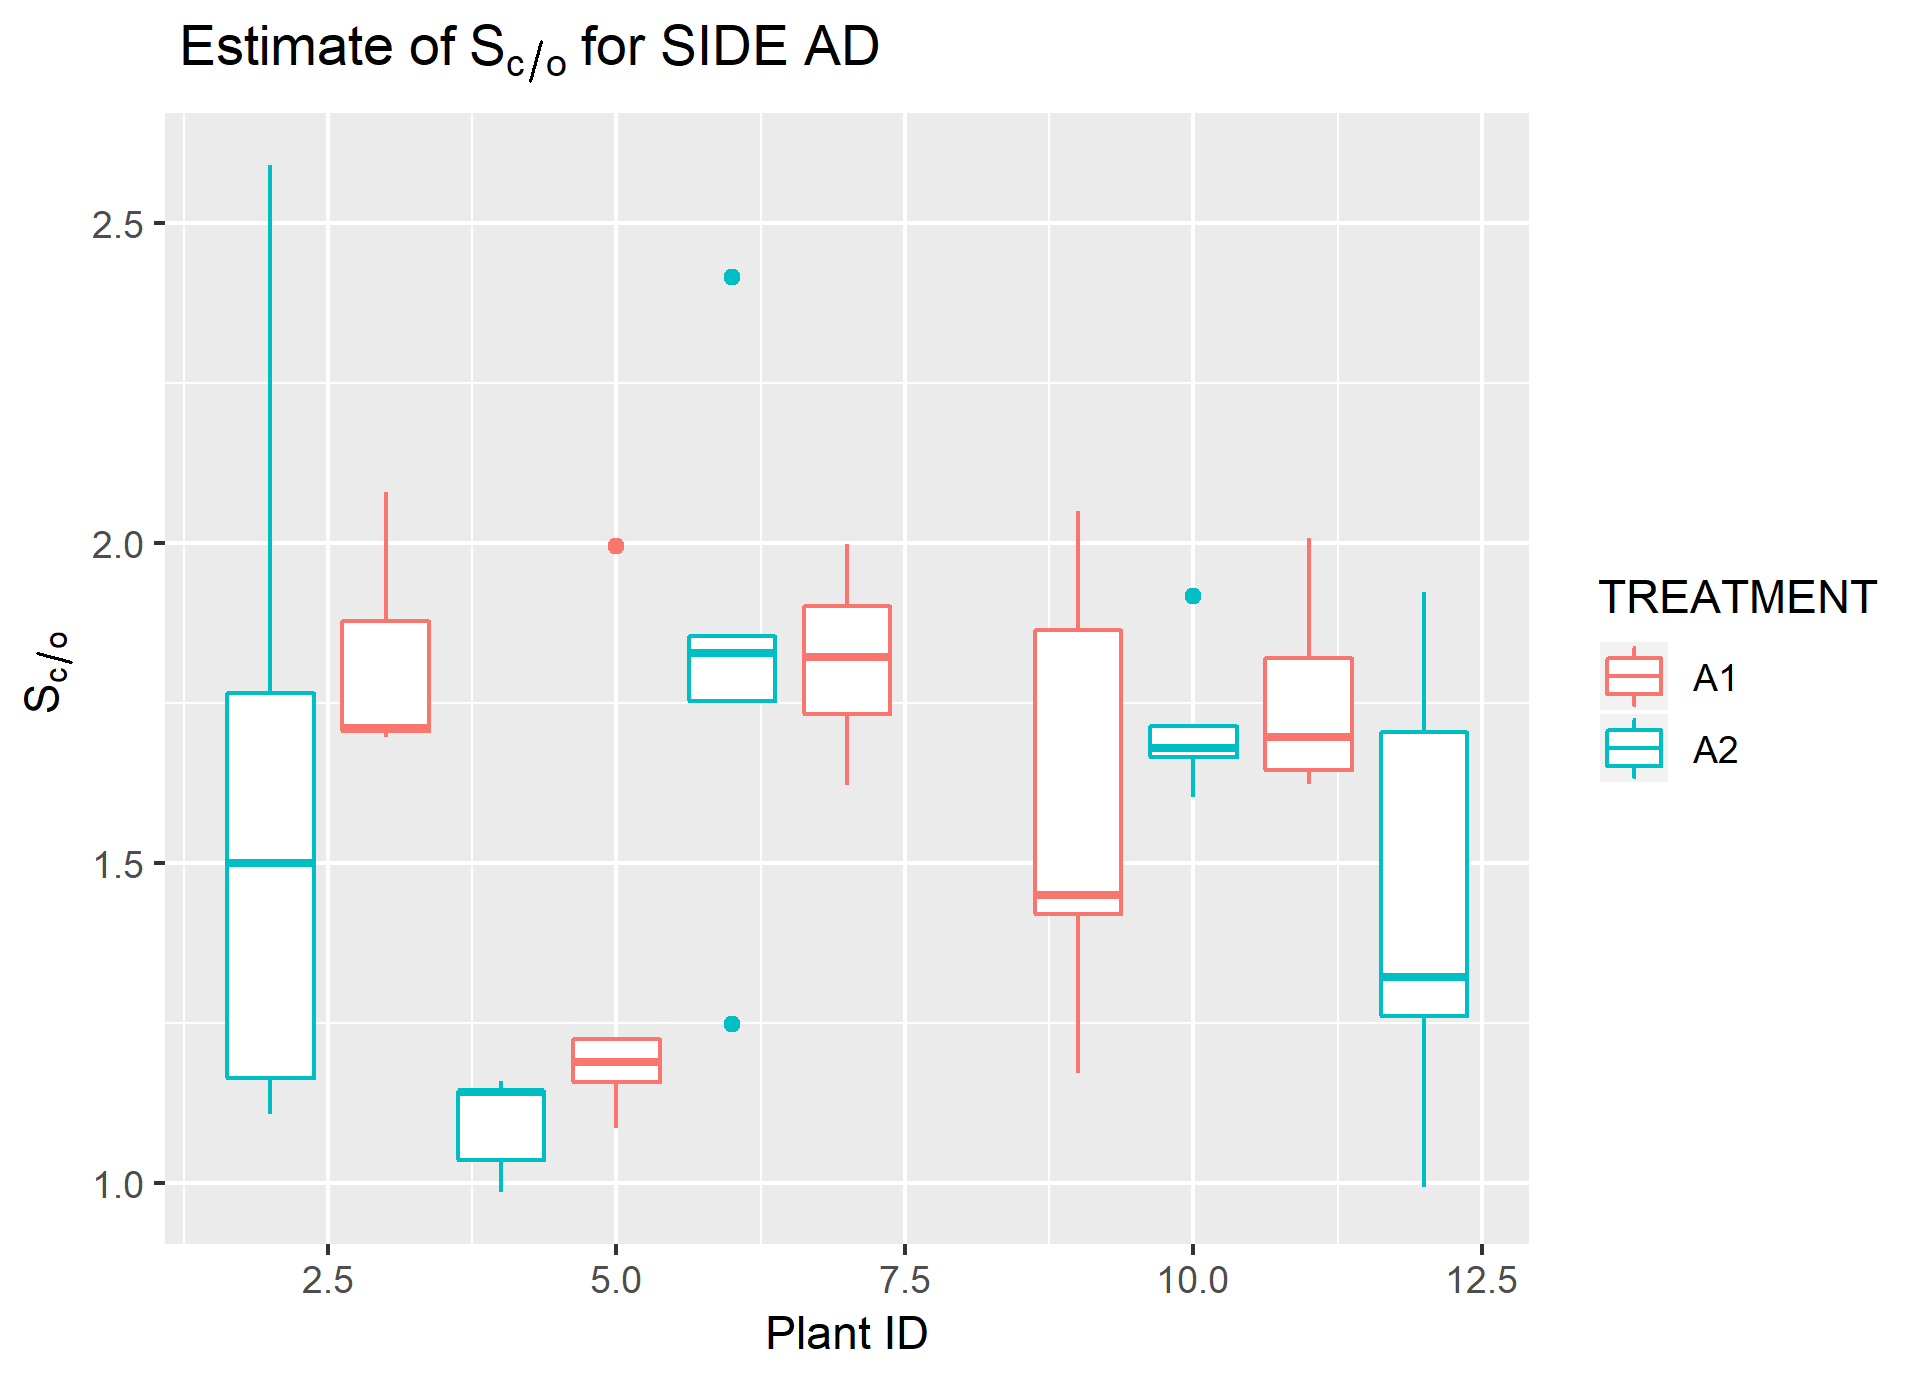
\includegraphics[scale=0.75]{Images/sco_boxplot_ad}
\caption{Range of values for $S_{c/o}$ for side measurement of AD.}
\label{fig:sco_ad}
\end{figure}

\subsection{$g_m$}
Using the previous results $g_m$ is estimated. We use a restricted range of $C_i \in [250, 300]$ based on conversation with Elias Kaiser. This gives a median estimate of $g_m$ of $0.03$.

\subsection{Non linear fixed effects model}
We attempt to fit a non-linear fixed effect model using the values estimated and allowing $V_{c_{max}}, J_{max}$ and $\theta$  to vary. Our results for the combinations of side and treatment (A1, AB) and (A2, AD) are found in table \ref{params_nls_est}; other side and treatment combinations could not converge.
\ctable[
cap = nls_parameters, botcap,
caption = {Estimate of parameters, $R_d$ and $s$, using fixed effect models},% \cite{CaemmererBiochemicalmodelsleaf2000}},
label = nowidth,
pos = !htb,
label = params_nls_est
] {cccccccc} {} { \FL
Side & Treatment & $V_{c_{max}}$ & $V_{c_{max}}$ s.e. & $J_{max}$ & $J_{max}$ s.e. & $\theta$ & $\theta$ s.e \ML
AB & A1 & 53.54 & 1.94 & 166.153 & 212.99 & -3.75 & 12.23 \NN
AD & A2 & 44.38 & 2.90 & 192.00 & 300.98 & -9.25 & 26.29 \ML
}

\subsection{Non-linear mixed effects model}
Unfortunately no on-linear mixed effects models could converge, so we have no results for this section.

\section{Conclusion and recommendations}
If we consider the results here, the values of $S_{c/o}$ are approximately half the expected value based upon the literature, $g_m$ is an order of magnitude smaller than what we expect to see. This suggests our analysis is flawed or else that these plants differ more from generic $C_3$ species than expected. We expect that the analysis being flawed would partially explain why no nlme model would converge, giving no estimates of the value for $V_{c_{max}}$ or $J_{max}$. Based on figure \ref{fig:lme_rd}, $R_d$ is more strongly affected by side than treatment, as is $s$ (see table \ref{params_est} and figure \ref{fig:lme_s}) and $S_{c/o}$ (see table \ref{sco_median} and figures \ref{fig:sco_ab} and \ref{fig:sco_ad}). However, as our results are strange and limited we have not implemented a full analysis.

The main realisation of this project is that there is a severe lack of transparency in the field of plant physiology. Different modelling techniques and underlying, unstated assumptions mean that many papers cannot be directly compared in their results. As a small example of unstated assumptions, no paper we read explicitly stated accounting for the Kok effect, however it appears to be standard practice based on correspondence and conversation with plant scientists. This is a serious flaw, as many models use the same name (i.e. the FvCB model), but actually refer to different versions. Beyond this all examples we could find in the literature use models that do not account for correlation within the data despite the use of repeated measurements (another unwritten assumption). This, coupled with a lack of reporting of errors on parameter estimates, leaves many published results highly opaque. Consider the table \ref{params_nls_est}. Here the point estimates of $V_{c_{max}}$ and $J_{max}$ appear sensible in comparison with the published literature. However, the error on $J_{max}$ is so large as to disfigure the result entirely. Furthermore, $\theta$ is negative (which is not expected) and also has a large error. If this result is not unique to this paper, many published results become questionable. Without explicit statement of the error on these estimates it is hard to comment on them.

With so many parameters, with so many methods available (either for estimating photosynthetic parameters as mentioned above or in estimating the Michaelis-Menten constants) and an understanding that dropping certain data points is dependent solely upon the modeler's discretion (which points are under the Kok effect, which points are part of the linear part of the ACI and LCR curves) it leaves the final results difficult to interpret. Arguably there is sufficient room to play with choices of relevant data, models used, auxiliary parameters to ensure that the point estimates found for the key parameters are within a reasonable distance of those previously published. We do not know if this flexibility is taken advantage of to produce results that are ``sensible'', but it does create difficulty in reproducing results or recreating a given method. We recommend that plant scientists be explicit in their modelling assumptions, in their data selection and in their estimated error values. A thorough review paper comparing the performance of different variations of the FvCB model, and within each model comparing the use of mixed effect and fixed effect models could be of great interest. If such a paper included error estimations and an explicit statement of the assumptions and data selection process for each model, it could be of great benefit.

As there is a lack of sufficient data and there exists strong domain knowledge, we also recommend use of Bayesian methods. Using a model such as that described by \citet{YinUsingcombinedmeasurements2009} also allows one to use the initial steps to produce priors on the parameters such as $s$ and $R_d$ while allowing the model to fit all variables simultaneously as in the work published by \citet{QianEstimationphotosynthesisparameters2012}. This would be advantageous as there is greater flexibility in fitting all of the parameters simultaneously and also the error associated with each parameters is present in the final model. Furthermore, the Bayesian methods allow principled quantification of the uncertainty associated with each parameter, not only is the credible range on the parameter included, but we have the full posterior distribution. The main problem that we foresee is that with the paucity of data it is possible that final model could be dominated by our priors; however if these priors are fed from other datasets from the same experiment (as in \cite{YinUsingcombinedmeasurements2009}) we suspect that this is still an improvement on the current approach.

%As the mechanistic model underlying the data is well understood, simulating data should be feasible if known is available (we understand that producing sufficient data for a single experiment can take up to a year's work and that plant scientists might be unwilling to share such results). 

\newpage

\bibliographystyle{plainnat}
\bibliography{thesis_ref}

\newpage

\appendix
\section{Linear light curves} \label{appendix:lcr_linear}
We include plots of the light response curves to show which points are relevant to the linear part of the curve and not influenced by the Kok effect.

\begin{figure}[h]
\centering
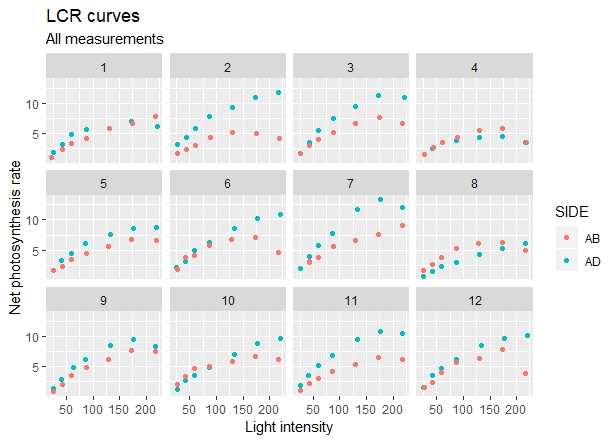
\includegraphics[scale=0.85]{Images/lcr_curves_all_low_o2}
\caption{LCR.}
\label{fig:lcr_curves_all_low_o2}
\end{figure}

\begin{figure}[h]
\centering
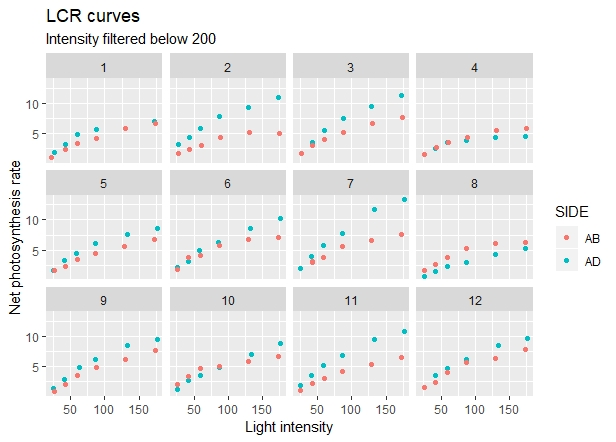
\includegraphics[scale=0.85]{Images/lcr_curves_b200_low_o2}
\caption{LCR.}
\label{fig:lcr_curves_b200_low_o2}
\end{figure}

\begin{figure}[h]
\centering
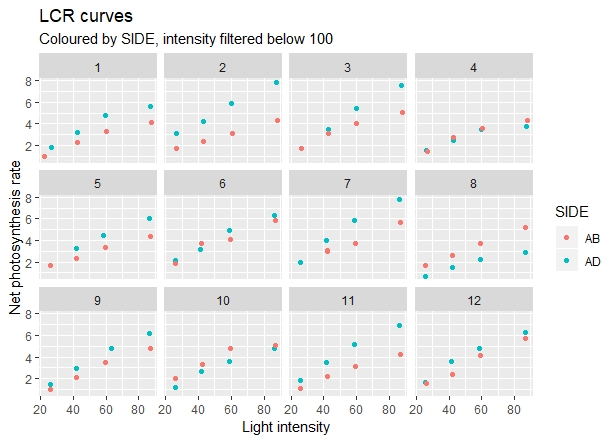
\includegraphics[scale=0.85]{Images/lcr_curves_b100_low_o2}
\caption{LCR.}
\label{fig:lcr_curves_b100_low_o2}
\end{figure}

\begin{figure}[h]
\centering
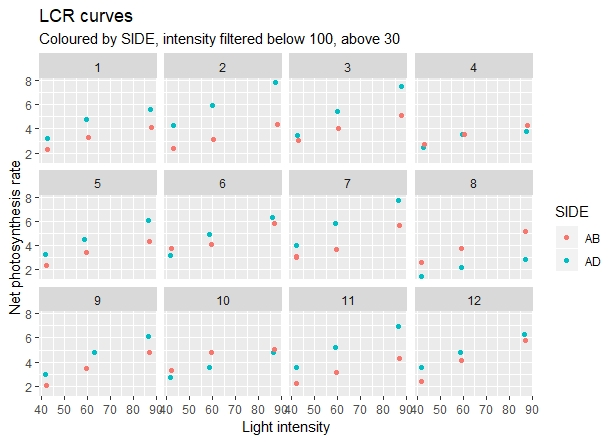
\includegraphics[scale=0.85]{Images/lcr_curves_b100_a30_low_o2}
\caption{LCR.}
\label{fig:lcr_curves_b100_a30_low_o2}
\end{figure}

\end{document}
